\begin{center}

\begin{tikzpicture}[font=\small,overlay,
mycirclex/.style={draw, circle, minimum size=1.0em, inner sep = 0.2mm}, 
mydiamond/.style={draw, diamond, minimum size=0.78em, inner sep = 0mm}, 
myrectang/.style={rounded corners, draw, rectangle, minimum size=0.60em, inner sep = 0.8mm, line width = 0.03cm}, 
>=stealth]

\def\cola{blue} 
\def\colb{orange}
\def\colc{mygreen}
\def\cold{purple} 
\def\cole{gray} 
\def\colf{cyan}
\def\colg{brown}


\def\len{1.65cm}

% G1
\begin{scope}[local bounding box=bbox, xshift=-6.9cm, yscale=1.2]
\path<2-> node[mycirclex] (v1) at (1.0 * \len, 0) {$s$};
\path<2-> node[mycirclex] (v2) at (2.0 * \len, 0) {$a$};
\path<2-> node[mycirclex] (v3) at (3.0 * \len, 0) {$b$};
\path<2-> node[mycirclex] (v4) at (4.0 * \len, 0) {$c$};
\path<2-> node[mycirclex] (v5) at (5.0 * \len, 0) {$d$};
\path<2-> node[mycirclex] (v6) at (6.0 * \len, 0) {$t$};

\path<3-> [draw, opacity = 1.0, \cola, ->, line width=0.082cm] (v1) -- (v2);
\path<3-> [draw, opacity = 1.0, \cola, ->, line width=0.082cm] (v2) -- (v3);
\path<3-> [draw, opacity = 1.0, \cola, ->, line width=0.082cm] (v3) -- (v4);
\path<3-> [draw, opacity = 1.0, \cola, ->, line width=0.082cm] (v4) -- (v5);
\path<3-> [draw, opacity = 1.0, \cola, ->, line width=0.082cm] (v5) -- (v6);
\path<3-> node[myrectang, rounded corners, \cola] at (7.03 * \len, 0.0cm) {$a(P_1) = 2n~(\times 1)$};

\path<2-> [draw, \colx, ->, line width=0.02cm] (v1) -- (v2);
\path<2-> [draw, \colx, ->, line width=0.02cm] (v2) -- (v3);
\path<2-> [draw, \colx, ->, line width=0.02cm] (v3) -- (v4);
\path<2-> [draw, \colx, ->, line width=0.02cm] (v4) -- (v5);
\path<2-> [draw, \colx, ->, line width=0.02cm] (v5) -- (v6);

\path<2-> [draw, \colx, ->, line width=0.02cm, bend left = 50] (v1) to (v2);
\path<2-> [draw, \colx, ->, line width=0.02cm, bend left = 50] (v5) to (v6);
\path<2-> [draw, \colx, ->, line width=0.02cm, bend left = 30] (v1) to (v4);
\path<2-> [draw, \colx, ->, line width=0.02cm, bend left = 30] (v3) to (v6);

\path<2-> [draw, \colx, ->, line width=0.02cm, bend left =-20] (v2) to (v3);
\path<2-> [draw, \colx, ->, line width=0.02cm, bend left =-30] (v2) to (v3);
\path<2-> [draw, \colx, ->, line width=0.02cm, bend left =-40] (v2) to (v3);
\path<2-> [draw, \colx, ->, line width=0.02cm, bend left =-50] (v2) to (v3);
\path<2-> [draw, \colx, ->, line width=0.02cm, bend left =-20] (v4) to (v5);
\path<2-> [draw, \colx, ->, line width=0.02cm, bend left =-30] (v4) to (v5);
\path<2-> [draw, \colx, ->, line width=0.02cm, bend left =-40] (v4) to (v5);
\path<2-> [draw, \colx, ->, line width=0.02cm, bend left =-50] (v4) to (v5);


\path<2-> node at (1.5 * \len, 0.17cm) {$2n$};
\path<2-> node at (2.5 * \len, 0.17cm) {$2n$};
\path<2-> node at (3.5 * \len, 0.17cm) {$2n$};
\path<2-> node at (4.5 * \len, 0.17cm) {$2n$};
\path<2-> node at (5.5 * \len, 0.17cm) {$2n$};

\path<2-> node at (1.4 * \len, 0.62cm) {$n$};
\path<2-> node at (5.6 * \len, 0.62cm) {$n$};
\path<2-> node at (2.5 * \len, 0.96cm) {$n$};
\path<2-> node at (4.5 * \len, 0.96cm) {$n$};

\path<2-> node at (2.5 * \len, -0.65cm) {$n\times 1$};
\path<2-> node at (4.5 * \len, -0.65cm) {$n\times 1$};

\path<4-> [draw, line width = 0.1cm, ->] (3.5 * \len, -0.7cm) to node[label=right:{Residual Graph}]{} (3.5 * \len, -1.4cm);
\end{scope}

% G2
\begin{scope}[local bounding box=bbox, xshift=-6.9cm, yscale=1.2, yshift=-2.4cm]
\path<4-> node[mycirclex] (v1) at (1.0 * \len, 0) {$s$};
\path<4-> node[mycirclex] (v2) at (2.0 * \len, 0) {$a$};
\path<4-> node[mycirclex] (v3) at (3.0 * \len, 0) {$b$};
\path<4-> node[mycirclex] (v4) at (4.0 * \len, 0) {$c$};
\path<4-> node[mycirclex] (v5) at (5.0 * \len, 0) {$d$};
\path<4-> node[mycirclex] (v6) at (6.0 * \len, 0) {$t$};

\path<5-> [draw, \colb, opacity = 1.0, ->, line width=0.082cm, bend left = 30] (v1) to (v4);
\path<5-> [draw, \colb, opacity = 1.0, <-, line width=0.082cm] (v3) -- (v4);
\path<5-> [draw, \colb, opacity = 1.0, ->, line width=0.082cm, bend left = 30] (v3) to (v6);
\path<5-> node[myrectang, rounded corners, \colb] at (7.03 * \len, 0.0cm) {$a(P_2) = n~(\times 1)$};

\path<4-> [draw, \colx, <-, line width=0.02cm] (v1) -- (v2);
\path<4-> [draw, \colx, <-, line width=0.02cm] (v2) -- (v3);
\path<4-> [draw, \colx, <-, line width=0.02cm] (v3) -- (v4);
\path<4-> [draw, \colx, <-, line width=0.02cm] (v4) -- (v5);
\path<4-> [draw, \colx, <-, line width=0.02cm] (v5) -- (v6);

\path<4-> [draw, \colx, ->, line width=0.02cm, bend left = 50] (v1) to (v2);
\path<4-> [draw, \colx, ->, line width=0.02cm, bend left = 50] (v5) to (v6);
\path<4-> [draw, \colx, ->, line width=0.02cm, bend left = 30] (v1) to (v4);
\path<4-> [draw, \colx, ->, line width=0.02cm, bend left = 30] (v3) to (v6);

\path<4-> [draw, \colx, ->, line width=0.02cm, bend left =-20] (v2) to (v3);
\path<4-> [draw, \colx, ->, line width=0.02cm, bend left =-30] (v2) to (v3);
\path<4-> [draw, \colx, ->, line width=0.02cm, bend left =-40] (v2) to (v3);
\path<4-> [draw, \colx, ->, line width=0.02cm, bend left =-50] (v2) to (v3);
\path<4-> [draw, \colx, ->, line width=0.02cm, bend left =-20] (v4) to (v5);
\path<4-> [draw, \colx, ->, line width=0.02cm, bend left =-30] (v4) to (v5);
\path<4-> [draw, \colx, ->, line width=0.02cm, bend left =-40] (v4) to (v5);
\path<4-> [draw, \colx, ->, line width=0.02cm, bend left =-50] (v4) to (v5);


\path<4-> node at (1.5 * \len, 0.17cm) {$2n$};
\path<4-> node at (2.5 * \len, 0.17cm) {$2n$};
\path<4-> node at (3.5 * \len, 0.17cm) {$2n$};
\path<4-> node at (4.5 * \len, 0.17cm) {$2n$};
\path<4-> node at (5.5 * \len, 0.17cm) {$2n$};

\path<4-> node at (1.4 * \len, 0.62cm) {$n$};
\path<4-> node at (5.6 * \len, 0.62cm) {$n$};
\path<4-> node at (2.5 * \len, 0.96cm) {$n$};
\path<4-> node at (4.5 * \len, 0.96cm) {$n$};

\path<4-> node at (2.5 * \len, -0.65cm) {$n\times 1$};
\path<4-> node at (4.5 * \len, -0.65cm) {$n\times 1$};
\path<6-> [draw, line width = 0.1cm, ->] (3.5 * \len, -0.7cm) to node[label=right:{Residual Graph}]{} (3.5 * \len, -1.4cm);
\end{scope}

% G3
\begin{scope}[local bounding box=bbox, xshift=-6.9cm, yscale=1.2, yshift=-4.8cm]
\path<6-> node[mycirclex] (v1) at (1.0 * \len, 0) {$s$};
\path<6-> node[mycirclex] (v2) at (2.0 * \len, 0) {$a$};
\path<6-> node[mycirclex] (v3) at (3.0 * \len, 0) {$b$};
\path<6-> node[mycirclex] (v4) at (4.0 * \len, 0) {$c$};
\path<6-> node[mycirclex] (v5) at (5.0 * \len, 0) {$d$};
\path<6-> node[mycirclex] (v6) at (6.0 * \len, 0) {$t$};

\path<7-> [draw, \cold, ->, line width=0.082cm, bend left = 50] (v1) to (v2);
\path<7-> [draw, \cold, ->, line width=0.082cm, bend left =-20] (v2) to (v3);
\path<7-> [draw, \cold, ->, line width=0.082cm, bend left = 10] (v3) to (v4);
\path<7-> [draw, \cold, ->, line width=0.082cm, bend left =-20] (v4) to (v5);
\path<7-> [draw, \cold, ->, line width=0.082cm, bend left = 50] (v5) to (v6);
\path<7-> node[myrectang, rounded corners, \cold] at (7.03 * \len, 0.0cm) {$a(P_3) = 1~(\times n)$};

\path<6-> [draw, \colx, <-, line width=0.02cm] (v1) -- (v2);
\path<6-> [draw, \colx, <-, line width=0.02cm] (v2) -- (v3);
\path<6-> [draw, \colx, <-, line width=0.02cm] (v4) -- (v5);
\path<6-> [draw, \colx, <-, line width=0.02cm] (v5) -- (v6);

\path<6-> [draw, \colx, ->, line width=0.02cm, bend left = 10] (v3) to (v4);
\path<6-> [draw, \colx, <-, line width=0.02cm, bend left =-10] (v3) to (v4);

\path<6-> [draw, \colx, ->, line width=0.02cm, bend left = 50] (v1) to (v2);
\path<6-> [draw, \colx, ->, line width=0.02cm, bend left = 50] (v5) to (v6);
\path<6-> [draw, \colx, <-, line width=0.02cm, bend left = 30] (v1) to (v4);
\path<6-> [draw, \colx, <-, line width=0.02cm, bend left = 30] (v3) to (v6);

\path<6-> [draw, \colx, ->, line width=0.02cm, bend left =-20] (v2) to (v3);
\path<6-> [draw, \colx, ->, line width=0.02cm, bend left =-30] (v2) to (v3);
\path<6-> [draw, \colx, ->, line width=0.02cm, bend left =-40] (v2) to (v3);
\path<6-> [draw, \colx, ->, line width=0.02cm, bend left =-50] (v2) to (v3);
\path<6-> [draw, \colx, ->, line width=0.02cm, bend left =-20] (v4) to (v5);
\path<6-> [draw, \colx, ->, line width=0.02cm, bend left =-30] (v4) to (v5);
\path<6-> [draw, \colx, ->, line width=0.02cm, bend left =-40] (v4) to (v5);
\path<6-> [draw, \colx, ->, line width=0.02cm, bend left =-50] (v4) to (v5);


\path<6-> node at (1.5 * \len, 0.17cm) {$2n$};
\path<6-> node at (2.5 * \len, 0.17cm) {$2n$};
\path<6-> node at (4.5 * \len, 0.17cm) {$2n$};
\path<6-> node at (5.5 * \len, 0.17cm) {$2n$};

\path<6-> node at (3.5 * \len, 0.2cm) {$n$};
\path<6-> node at (3.5 * \len, -0.2cm) {$n$};

\path<6-> node at (1.4 * \len, 0.62cm) {$n$};
\path<6-> node at (5.6 * \len, 0.62cm) {$n$};
\path<6-> node at (2.5 * \len, 0.96cm) {$n$};
\path<6-> node at (4.5 * \len, 0.96cm) {$n$};

\path<6-> node at (2.5 * \len, -0.65cm) {$n\times 1$};
\path<6-> node at (4.5 * \len, -0.65cm) {$n\times 1$};
\end{scope}



\end{tikzpicture}
\end{center}
